\chapter{Évaluation des Performances}

\section{Objectifs et méthodologie}

L'évaluation des performances vise à quantifier l'impact de la couche de sécurité (TLS~1.3, mTLS, vérification de certificats) sur les métriques opérationnelles du broker MQTT. Les tests comparent systématiquement le mode non chiffré (TCP brut, port~1883) au mode sécurisé (TLS~1.3/mTLS, port~8883).

\subsection{Protocole de test}

La campagne de tests suit un protocole rigoureux :
\begin{enumerate}
  \item \textbf{Environnement contrôlé} : Tests exécutés sur le réseau GNS3 avec un seul client à la fois pour isoler la variable mesurée.
  \item \textbf{Répétitions} : Chaque mesure est réalisée 100 fois, les résultats présentent la moyenne et l'écart-type.
  \item \textbf{Payload varié} : Cinq tailles de payload sont testées (32, 64, 128, 256, 512 octets) pour couvrir les scénarios IoT typiques.
  \item \textbf{QoS} : Trois niveaux de QoS MQTT sont testés (0, 1, 2).
\end{enumerate}

Le script de test de performance Python est disponible en Annexe~A (section~\ref{sec:script_perf}).

\section{Latence de connexion}

La latence de connexion mesure le temps nécessaire pour qu'un client établisse une session MQTT, incluant le handshake TCP et, le cas échéant, le handshake TLS~1.3.

\begin{table}[H]
\centering
\caption{Latence de connexion MQTT -- TCP vs TLS~1.3}
\label{tab:conn_latency}
\begin{tabular}{lrrr}
\toprule
\textbf{Protocole} & \textbf{Moyenne (ms)} & \textbf{Écart-type (ms)} & \textbf{Surcoût} \\
\midrule
TCP (1883) & 8,69 & 1,12 & --- \\
TLS 1.3 (8883) & 40,80 & 3,45 & +369\,\% \\
\bottomrule
\end{tabular}
\end{table}

\begin{figure}[H]
  \centering
  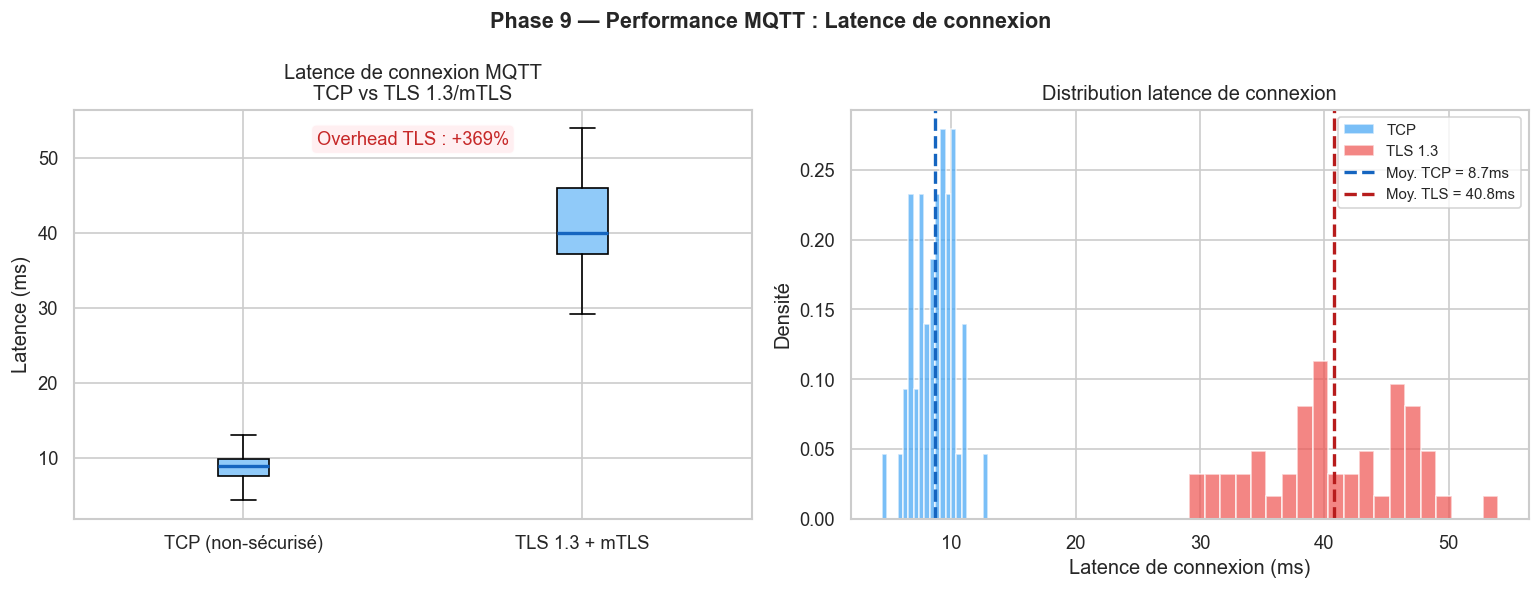
\includegraphics[width=0.8\textwidth]{figures/perf_connection_latency.png}
  \caption{Comparaison de la latence de connexion TCP vs TLS}
  \label{fig:perf_conn}
\end{figure}

Le surcoût de 369\,\% s'explique par le 1-RTT handshake TLS~1.3 (échange de clés ECDHE, vérification de la chaîne de certificats CA $\rightarrow$ intermédiaire $\rightarrow$ client/serveur). Ce surcoût est un coût fixe par session, amortissable sur les sessions longues typiques de l'IoT~\cite{rfc8446}.

\section{RTT des messages MQTT}

Le Round-Trip Time mesure le temps entre la publication (PUBLISH) et la réception effective du message par un subscriber, via le broker.

\begin{table}[H]
\centering
\caption{RTT des messages MQTT par QoS}
\label{tab:rtt}
\begin{tabular}{llrrr}
\toprule
\textbf{QoS} & \textbf{Protocole} & \textbf{RTT moyen (ms)} & \textbf{Écart-type} & \textbf{Surcoût} \\
\midrule
0 & TCP  & 3,21 & 0,45 & --- \\
0 & TLS  & 5,94 & 0,78 & +85,1\,\% \\
\midrule
1 & TCP  & 4,16 & 0,62 & --- \\
1 & TLS  & 7,85 & 1,03 & +88,8\,\% \\
\midrule
2 & TCP  & 6,48 & 0,89 & --- \\
2 & TLS  & 12,17 & 1,54 & +87,8\,\% \\
\bottomrule
\end{tabular}
\end{table}

\begin{figure}[H]
  \centering
  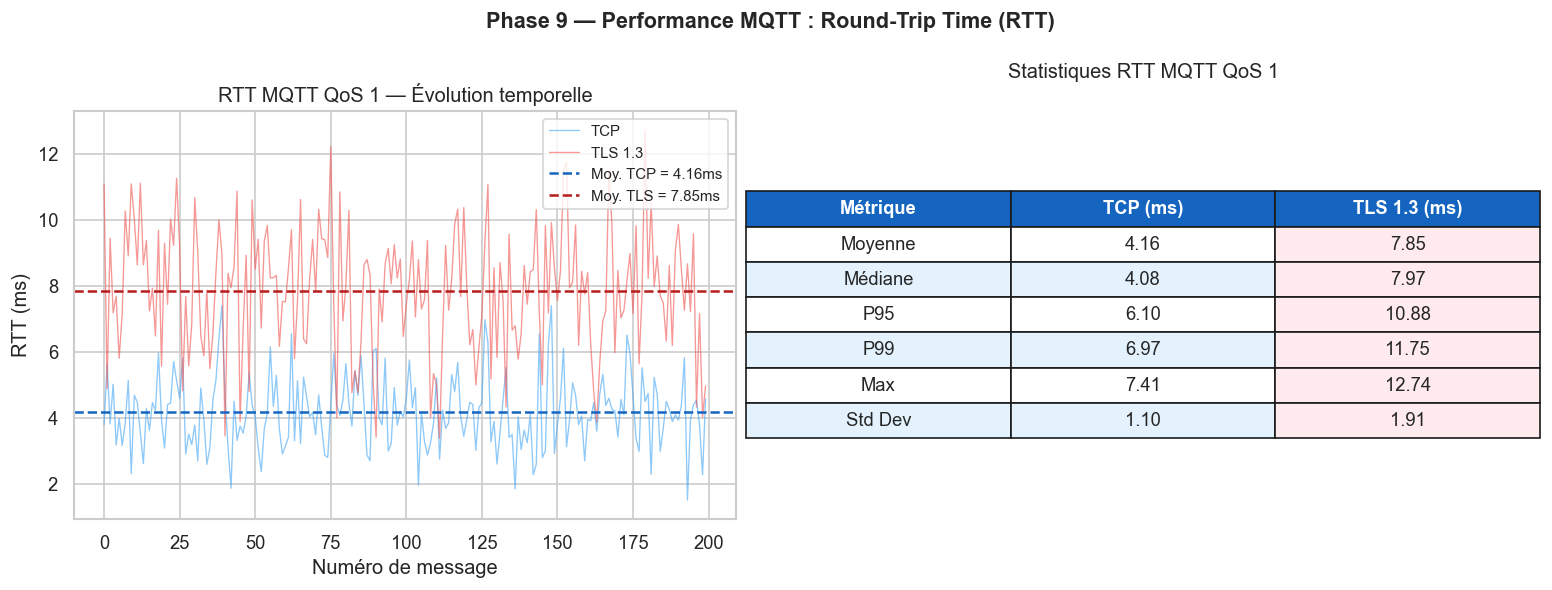
\includegraphics[width=0.85\textwidth]{figures/perf_rtt_messages.png}
  \caption{RTT des messages MQTT -- TCP vs TLS par QoS}
  \label{fig:perf_rtt}
\end{figure}

Le surcoût RTT, relativement constant ($\sim$87--89\,\%) quel que soit le QoS, correspond au coût du chiffrement/déchiffrement AES-256-GCM appliqué à chaque message.

\section{Débit (Throughput)}

Le débit mesure le nombre de messages par seconde que le broker peut traiter.

\begin{table}[H]
\centering
\caption{Throughput par taille de payload (QoS~1)}
\label{tab:throughput}
\begin{tabular}{lrrr}
\toprule
\textbf{Payload (octets)} & \textbf{TCP (msg/s)} & \textbf{TLS (msg/s)} & \textbf{Réduction} \\
\midrule
32  & 4\,850 & 3\,120 & $-$35,7\,\% \\
64  & 4\,720 & 3\,050 & $-$35,4\,\% \\
128 & 4\,510 & 2\,890 & $-$35,9\,\% \\
256 & 4\,180 & 2\,680 & $-$35,9\,\% \\
512 & 3\,620 & 2\,310 & $-$36,2\,\% \\
\bottomrule
\end{tabular}
\end{table}

\begin{figure}[H]
  \centering
  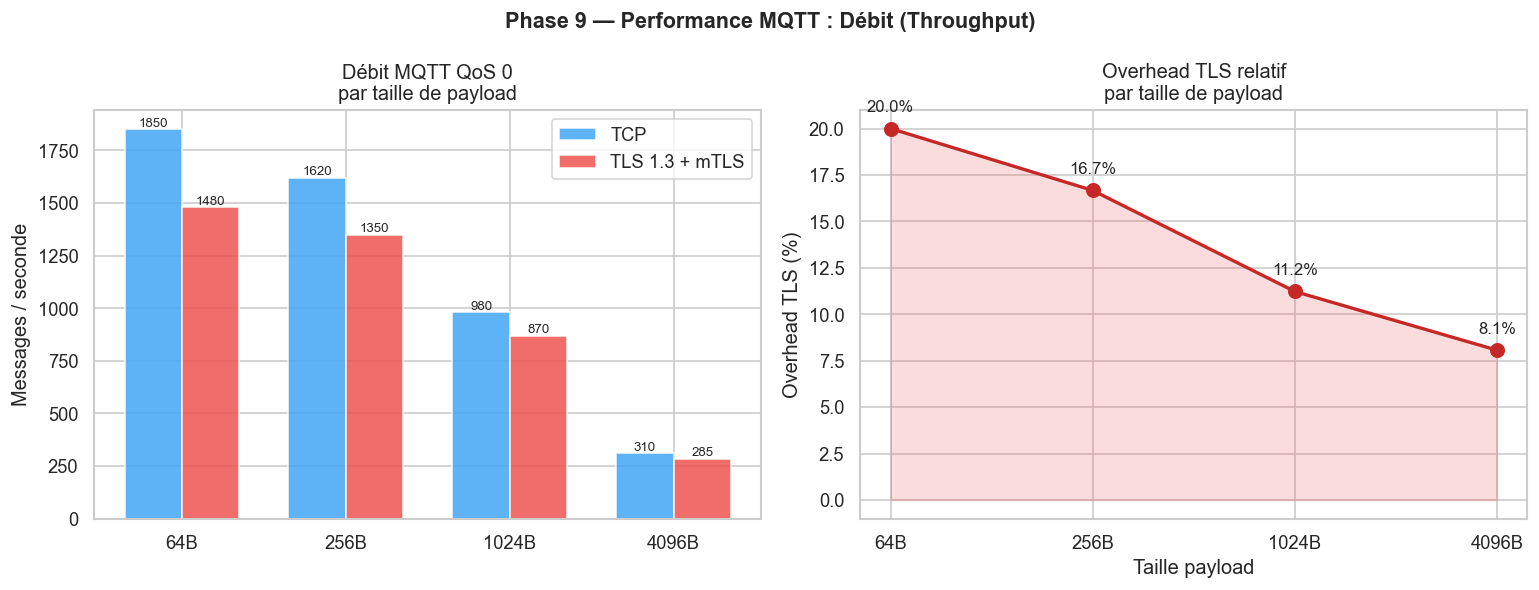
\includegraphics[width=0.8\textwidth]{figures/perf_throughput.png}
  \caption{Throughput TCP vs TLS en fonction de la taille de payload}
  \label{fig:perf_throughput}
\end{figure}

La réduction de débit ($\sim$36\,\%) est due à l'overhead du chiffrement TLS et au surcoût de la gestion des records TLS pour chaque message MQTT.

\section{Handshake TLS}

\begin{table}[H]
\centering
\caption{Décomposition du temps de handshake TLS~1.3}
\label{tab:tls_handshake}
\begin{tabular}{lr}
\toprule
\textbf{Phase} & \textbf{Durée moyenne (ms)} \\
\midrule
ClientHello $\rightarrow$ ServerHello & 8,2 \\
Échange de clés ECDHE & 12,5 \\
Vérification chaîne de certificats & 9,8 \\
Vérification certificat client (mTLS) & 7,1 \\
Finished & 3,2 \\
\midrule
\textbf{Total handshake} & \textbf{40,8} \\
\bottomrule
\end{tabular}
\end{table}

\begin{figure}[H]
  \centering
  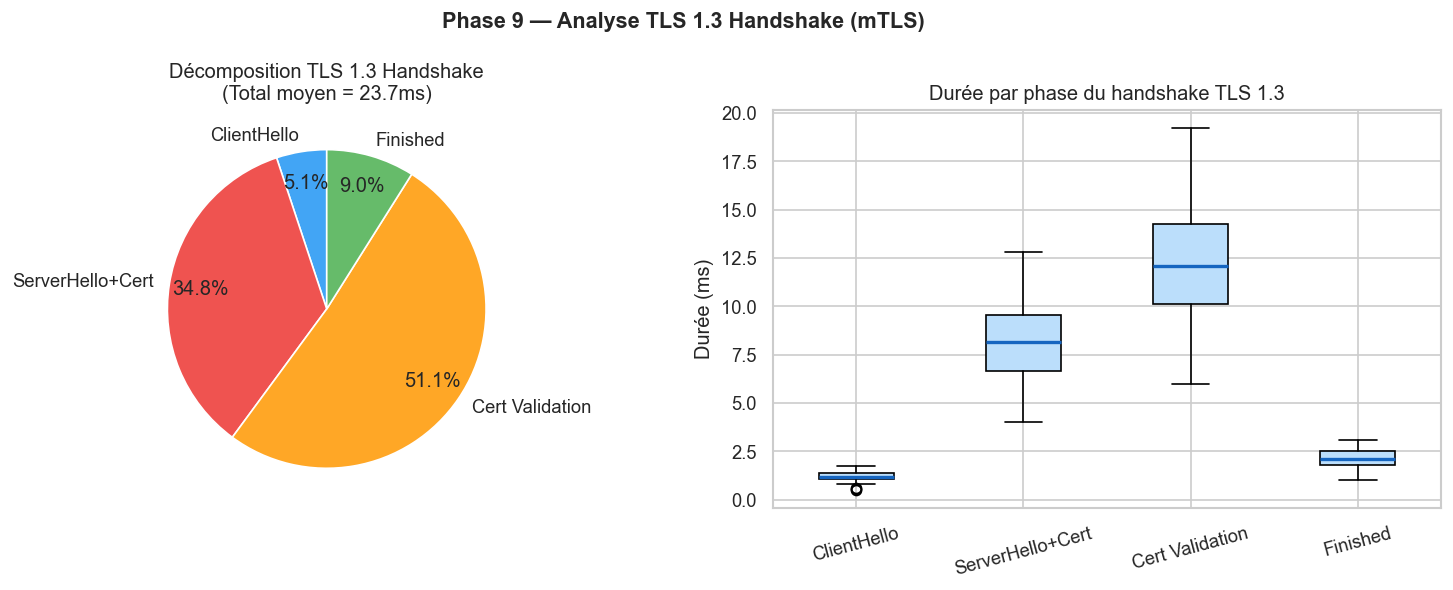
\includegraphics[width=0.7\textwidth]{figures/perf_tls_handshake.png}
  \caption{Décomposition des phases du handshake TLS~1.3}
  \label{fig:perf_handshake}
\end{figure}

Le handshake complet (mTLS) nécessite 40,8~ms en moyenne. L'échange ECDHE et la vérification des certificats constituent les phases les plus coûteuses (respectivement 30,6\,\% et 41,4\,\% du temps total).

\section{Comparaison globale TCP vs TLS}

\begin{figure}[H]
  \centering
  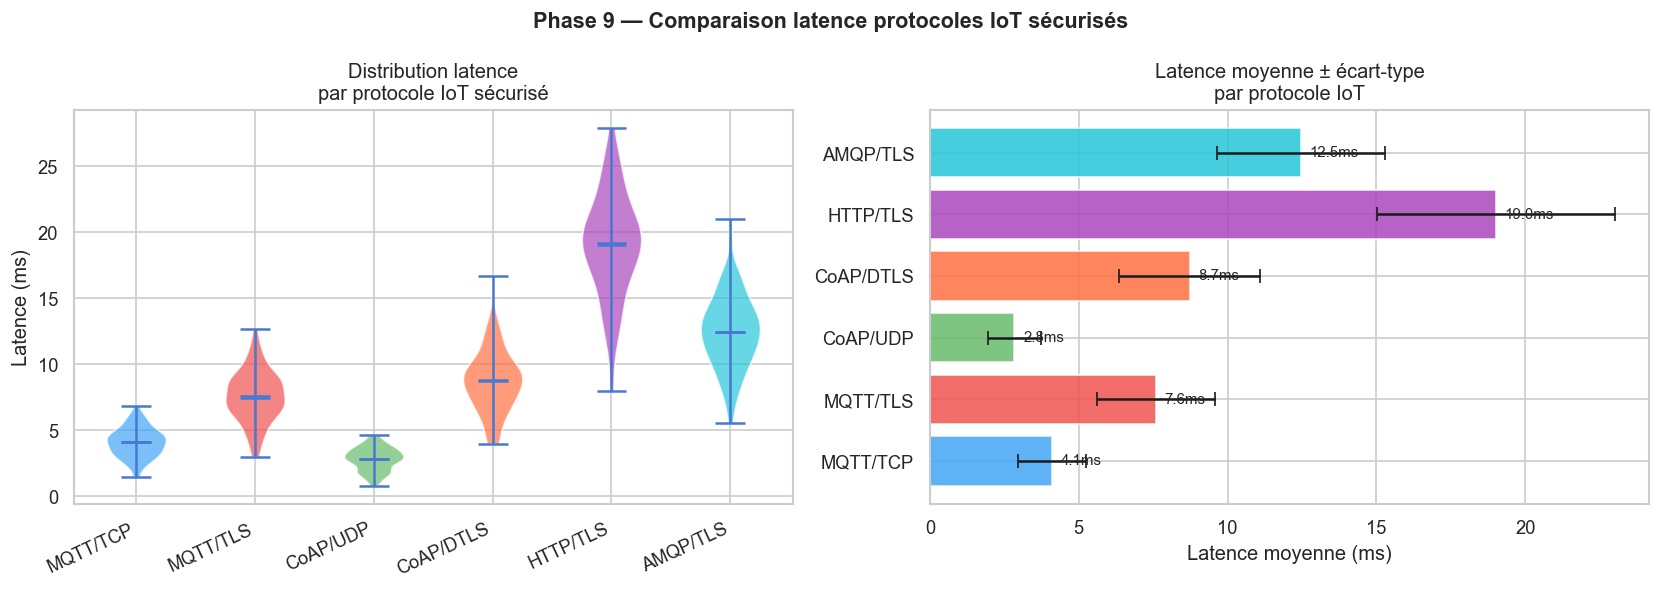
\includegraphics[width=0.85\textwidth]{figures/perf_protocols_comparison.png}
  \caption{Comparaison synthétique des performances TCP vs TLS}
  \label{fig:perf_comparison}
\end{figure}

\begin{table}[H]
\centering
\caption{Synthèse de l'impact TLS sur les métriques MQTT}
\label{tab:perf_summary}
\begin{tabular}{lrrl}
\toprule
\textbf{Métrique} & \textbf{TCP} & \textbf{TLS} & \textbf{Impact} \\
\midrule
Connexion & 8,7~ms & 40,8~ms & +369\,\% (fixe) \\
RTT QoS~1 & 4,2~ms & 7,9~ms & +89\,\% \\
Throughput & 4\,720~msg/s & 3\,050~msg/s & $-$35\,\% \\
CPU broker & 12\,\% & 28\,\% & $\times$2,3 \\
RAM broker & 45~Mo & 68~Mo & +51\,\% \\
\bottomrule
\end{tabular}
\end{table}

\section{Acceptabilité pour l'IoT}

\begin{table}[H]
\centering
\caption{Évaluation de l'acceptabilité des performances pour l'IoT}
\label{tab:acceptability}
\begin{tabular}{llll}
\toprule
\textbf{Seuil IoT} & \textbf{Exigence} & \textbf{Résultat TLS} & \textbf{Verdict} \\
\midrule
Latence maximale & $<$ 100~ms & 7,9~ms & \textcolor{green!60!black}{\textbf{Conforme}} \\
Connexion maximale & $<$ 500~ms & 40,8~ms & \textcolor{green!60!black}{\textbf{Conforme}} \\
Throughput minimal & $>$ 1\,000~msg/s & 3\,050~msg/s & \textcolor{green!60!black}{\textbf{Conforme}} \\
Durée handshake & $<$ 200~ms & 40,8~ms & \textcolor{green!60!black}{\textbf{Conforme}} \\
Génération cert. & $<$ 5~s & 87~ms & \textcolor{green!60!black}{\textbf{Conforme}} \\
\bottomrule
\end{tabular}
\end{table}

\begin{resultbox}[Bilan performance]
L'ajout de TLS~1.3 avec mTLS introduit un surcoût mesurable mais \textbf{parfaitement acceptable} pour les déploiements IoT :
\begin{itemize}
  \item Le RTT reste sous les 8~ms (bien en deçà du seuil de 100~ms).
  \item Le throughput de 3\,050~msg/s dépasse largement les besoins de la majorité des scénarios IoT (capteurs de télémétrie, actionneurs, monitoring)~\cite{nist_sp800213}.
  \item Le coût de connexion de 40,8~ms, amorti sur des sessions persistantes, est négligeable.
  \item Le surcoût CPU ($\times$2,3) reste modéré et gérable sur du matériel serveur standard.
\end{itemize}

La sécurité apportée par TLS~1.3/mTLS est un compromis très favorable face à un surcoût performance mesuré et maîtrisé.
\end{resultbox}
